\documentclass[12pt]{article}
\setlength{\oddsidemargin}{27mm}
\setlength{\evensidemargin}{27mm}
\setlength{\hoffset}{-1in}

\usepackage{graphicx}
\usepackage{hyperref}
\usepackage[english]{babel}

\usepackage{apacite}

\setlength{\topmargin}{27mm}
\setlength{\voffset}{-1in}
\setlength{\headheight}{0pt}
\setlength{\headsep}{0pt}

\setlength{\textheight}{235mm}
\setlength{\textwidth}{155mm}

%\pagestyle{empty}
\pagestyle{plain}

\renewcommand{\thefootnote}{\fnsymbol{footnote}}
\renewcommand{\labelitemi}{$\diamond$}

\begin{document}
\baselineskip 12pt

\begin{center}
\textbf{\large Exploring the Dynamics of COVID-19 Spread Using a Generalized Lotka-Volterra Model (gLV)\\ } 

\vspace{1.5cc}
{ \sc Jay Hwasung Jung$^{1}$}\\

\vspace{0.3 cm}

{\small $^{1}$Computer Science B.S., University of Vermont  \\ \href{https://github.com/marszzibros/CSYS296}{https://github.com/marszzibros/CSYS296}
}

 \end{center}

% abstract
\begin{abstract}
COVID-19, also known as SARS-CoV-2, is a highly contagious respiratory illness that has had a significant global impact since it was first detected in Wuhan, China, in 2019. Its severe symptoms have posed a threat to public health, and various governmental regulations, such as quarantining, masking, and hand-washing, have been suggested and evaluated to mitigate the threat \cite{haug_2020_ranking}. However, the pandemic's duration has been a matter of public concern as it has persisted for over three years. To predict and estimate the pandemic's end, several methods have been suggested, such as the statistical power series model and the generalized Lokta-Volterra model (gLV). Although the statistical power series model can estimate the number of confirmed infected people, it cannot account for essential factors like immigration or infection rates \cite{baniyounes_2020_covid19}. In their paper, Younes and Hasan (2020) used gLV, an ecological model that simulates the interaction dynamics of multiple species, to simulate the interaction dynamics of COVID-19's populations (healthy and infected). gLV is a widely used ecological model that explains interaction dynamics between more than two species and has been used to analyze gut microbiome communities (Venturelli et al., 2018)\cite{venturelli_2018_deciphering}. Younes and Hasan (2020) attempted to predict COVID-19's behavior from the early stages, and according to their analysis, the infection rate ($\beta$) was critical to the dynamics. The review also implemented control sections not implemented in the original paper. The results suggest that COVID-19 will not be eradicated but will stabilize over time and live within populations.

\vspace{0.95cc}
\parbox{24cc}{{\it COVID-19, Generalized Lotka-Volterra (gLV), Data Analysis, Computational Systems Biology}:%Fill maximum 5 key words
}

\end{abstract}


\pagebreak

% background
\section{Background} \label{form}
\hspace{5mm}SARS-CoV-2, also known as COVID-19, is a highly infectious respiratory disease that has significantly impacted human activity worldwide since the first case was reported in Wuhan, China, in 2019. The virus is primarily spread through respiratory droplets, making it a significant public health concern. As a result, many governments worldwide have implemented regulatory measures to control the spread of the virus. These measures include social distancing, wearing masks, and lockdowns (Haug et al., 2020). To reduce the impacts of COVID-19 on public health, not only such controls but also vaccines and cures have been developed and authorized for emergency use in many countries. Although there has been a lot of efforts to control the spread and normalize our life, the end of the pandemic is still unclear. As a result, many experts and researchers came up with the methods (i.e. Machine Learning) to predict when the pandemic will end based on the accumulated data since 2019. 

One method introduced by Younes and Hasan (2020) is to build a Generalized Lotka-Volterra (gLV) dynamic model. gLV dynamic models allow us to investigate and understand the complex interactions between populations within ecological communities. By mathematically modeling the relationships between species, these models enable us to explore how different ecological factors, such as competition and predation, impact the dynamics of populations over time. Due to the advantages that gLV has, it has been used to describe ecological interactions or phenomena.

In COVID-19 analysis using gLV (Younes and Hasan, 2020), two populations are used: (1) healthy populations and (2) infected populations. These two populations grow and diminish as they interact. For example, in the paper by Younes and Hasan (2020), they considered birth, immigration (travel), infection rate, recovery rate, death rate, and control (i.e., effectiveness of vaccines, hand washing). Following is the gLV model we will be using:
\vspace{-3mm}
\begin{center}
    
\includegraphics[width=10.5cm, 
height=1.8cm]{img/(1).png}
\end{center}
\vspace{-3mm}
The differential equations below show the population dynamics of two species considering these factors acquired by gLV above:

\vspace{5mm}
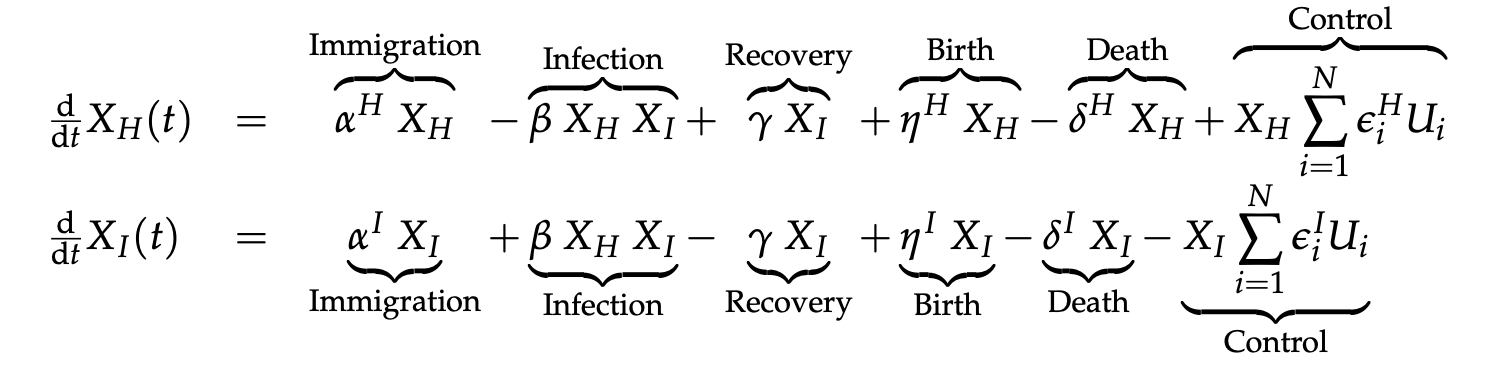
\includegraphics[width=14.5cm, height=3.7cm]{img/(2).png}
\vspace{5mm}

The variables $X_H(t)$ and $X_I(t)$ represent the healthy and infected populations over time $t$, respectively. The immigration rate, or travel rate, is denoted by $\alpha \geq 0$. If travel restrictions are imposed, $\alpha$ will be equal to 0. The infection rate is denoted by $\beta \geq 0$. In an ideal scenario where social distancing is ensured, $\beta$ will be 0. The recovery rate $\gamma$ is a fixed value of 25.5\% (the global average) in this paper. The birth and death rates are denoted by $\eta$ and $\delta$, respectively. The effectiveness of vaccines and treatments is represented by $\epsilon_H$ and $\epsilon_I$.

The control variable $u(x)$ includes border restrictions (53\%), active communication with healthcare professionals (11\%), increasing the healthcare workforce (35\%), increasing government support for vulnerable populations (41\%), and national lockdowns (25\%), as analyzed by Haug et al. (2020). 

\pagebreak

\section{Results} \label{subm}
\subsection{COVID-19 Spike Protein Structure}
\hspace{5mm} To begin with, understanding the structure of COVID-19 is essential to comprehend how it affects humans. The virus has a unique structure that includes a spike protein called 6VXX (Structure of the SARS-CoV-2 spike glycoprotein). The spike protein, also known as the S protein, plays a crucial role in the virus's receptor recognition and cell membrane fusion process. This protein is made up of two subunits, S1 and S2. The S1 subunit contains a receptor-binding domain that specifically binds to the host receptor angiotensin-converting enzyme 2. On the other hand, the S2 subunit facilitates viral cell membrane fusion through the formation of a six-helical bundle via the two-heptad repeat domain. Recent research advancements have shed light on the development of antiviral drugs that target the S protein (Huang et al., 2020). Fig 1 shows the simulated protein structure of the S protein of COVID-19.

\vspace{5mm}

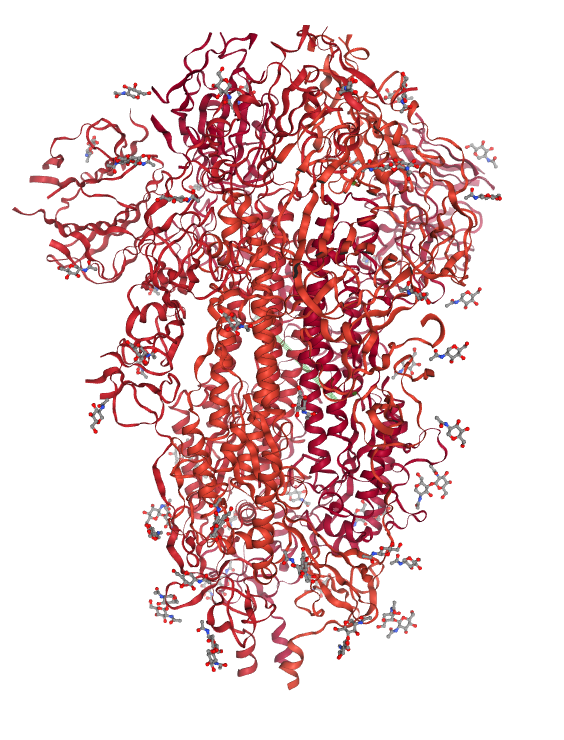
\includegraphics[width=6cm, height=6cm]{img/spike.png} 
\hspace{5mm}
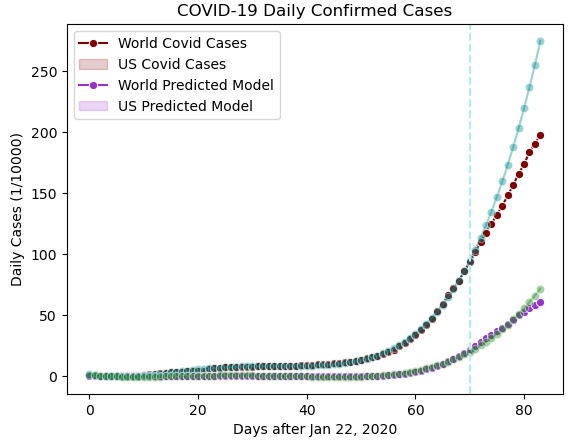
\includegraphics[width=8cm, height=6cm]{img/COVID19_confirmed.png}

Fig 1. 6VXX COVID-19 S protein \hspace{5mm}Fig 2. COVID-19 Confirmed Cases Prediction

\subsection{Statistical Analysis of COVID-19 Confirmed Cases}
\hspace{5mm} Figure 2 depicts the confirmed cases of COVID-19 provided by the WHO from January 22, 2020, to April 14, 2020. As the graph shows, the number of cases increases over time. It's important to note that this data was collected before the vaccine was developed and before many regulations were put in place.

\begin{center}
    \Large$\large y_j = \sum_{n=1}^N a_nt^n$; $j = 0,1,...,M$
\end{center}

The equation above shows the statistical power series model that I used to create Figure 2 after March 31, 2020. As shown, the prediction model is precise enough to estimate the future number of confirmed cases. However, it's important to note that this estimate is based on only three months of data and is not suitable for predicting the behavior of the infection in the long term. There are many unexpected factors that can influence infection rates, such as developments in vaccination and travel restrictions. While this model can provide an estimate of the number of COVID-19 patients, it's not suitable for describing the behavior of COVID-19.

\pagebreak
\subsection{Generalized Lokta-Volterra Model}
\hspace{5mm} As described in the background section, the generalized Lokta-Volterra (gLV) Model can simulate the ecological behaviors of many species. One well-known use of this model is to describe interactions within microbial communities (Venturelli1 et al., 2018). However, in the research conducted by Younes and Hasan (2020), the model was used to simulate the interactions between healthy and infected human populations. In their study, Younes and Hasan (2020) created a hypothetical country with a population of 100 people, consisting of 50 healthy individuals and 50 infected individuals. At the time of the study, no control measures were in place as there was no available data. In the optimal solution shown in Figure 03, no one travels or immigrates ($\alpha = 0$), resulting in a zero infection rate ($\beta = 0$). The recovery rate of 0.25 is based on the global average ($\gamma = 0.25$), while the birth and death rates are 0.01 and 0.001, respectively.

\vspace{5mm}
\hspace{-6mm}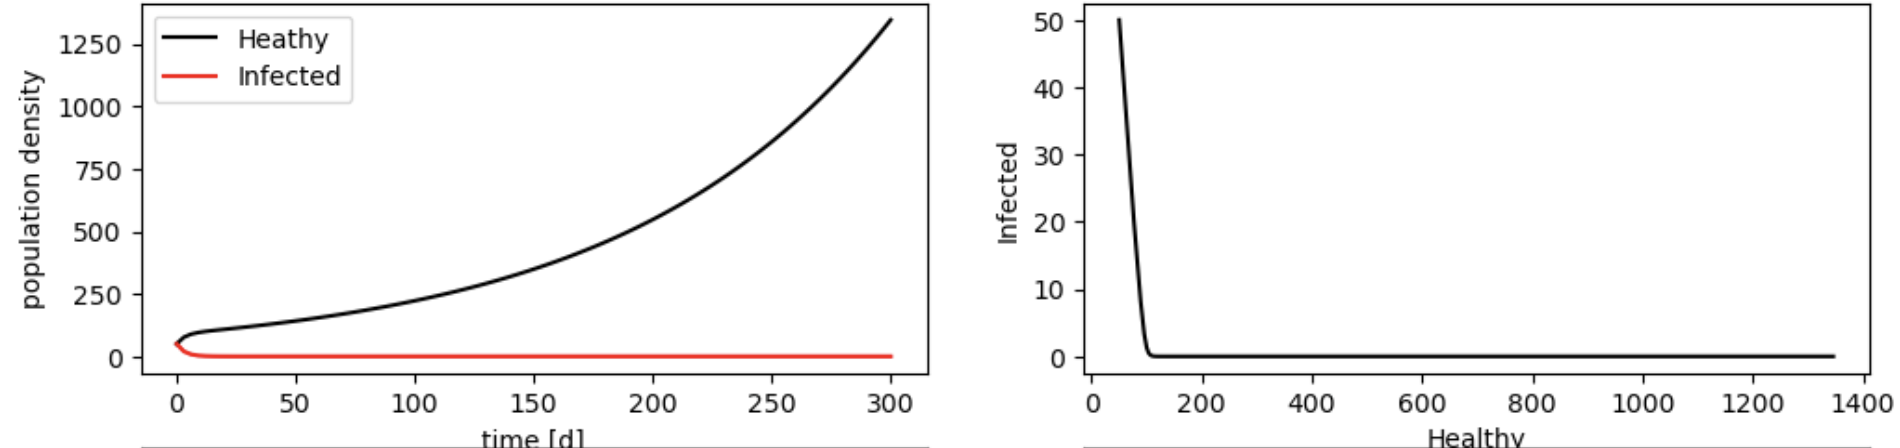
\includegraphics[width=16cm, height=5.2cm]{img/optimal_case.png}

\vspace{3mm}
\hspace{37mm} Figure 3. Optimal Case - No Immigration

\vspace{3mm}
Figure 3 shows that the number of infected people decreases in a short period of time, while the number of healthy individuals grows due to the birth rate. This could explain how the pandemic might have ended early if no one had been traveling.

\vspace{5mm}
\hspace{-6mm}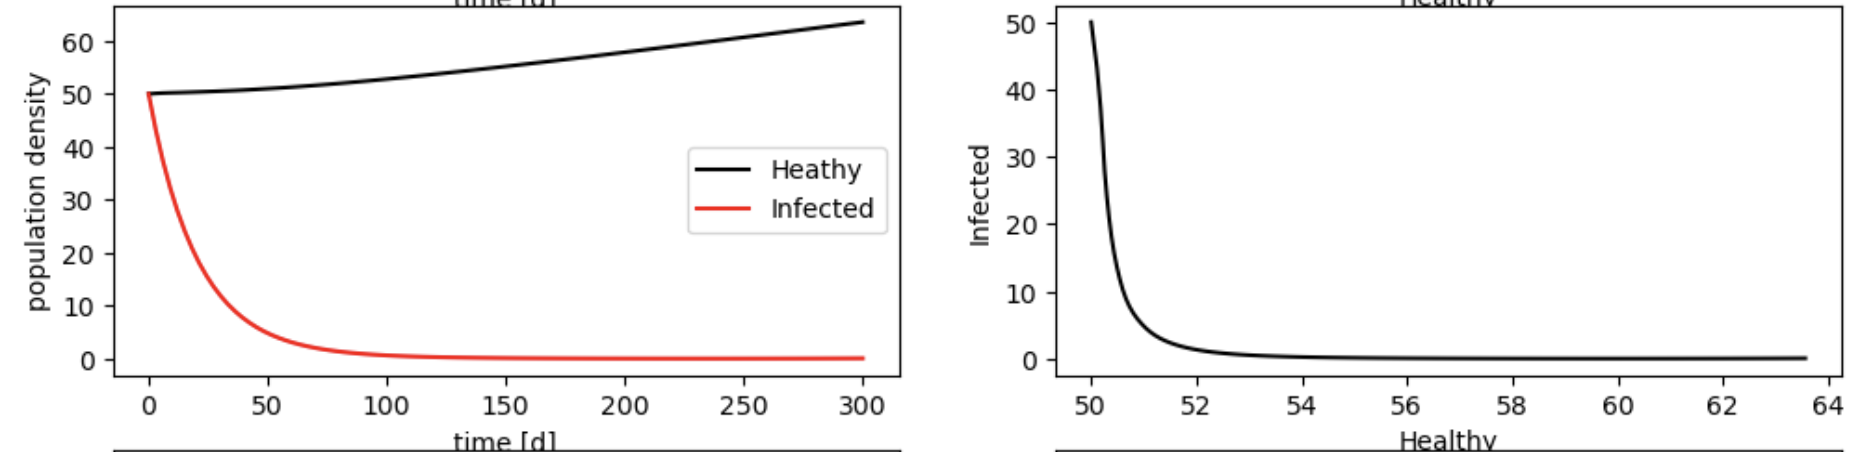
\includegraphics[width=16cm, height=5.2cm]{img/second_case_low_infection.png}

\vspace{5mm}
\hspace{37mm} Figure 4. Immigration 0.001 but Low Infection Rate
\vspace{5mm}

Figure 4 shows a graph of the immigration rate of 0.001 and an infection rate of 0.005. Although the decrease in the infected population is slower than in the optimal case (Figure 03), the infected population eventually reaches zero, and the pandemic comes to an end.


\hspace{-6mm}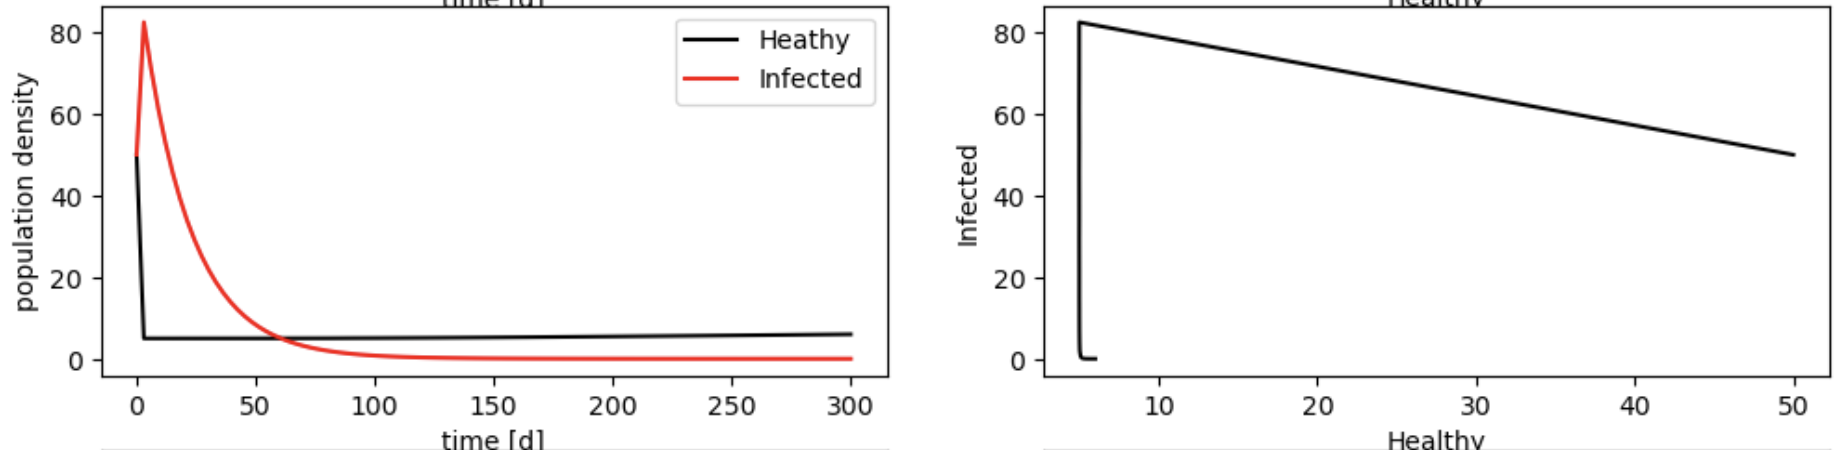
\includegraphics[width=16cm, height=5.2cm]{img/third_case_high_infection.png}

\vspace{3mm}
\hspace{30mm} Figure 5. Immigration 0.001 but a High Infection Rate

\vspace{3mm}

The conditions for Figure 05 are identical to those for Figure 04, except for the infection rate, which is 0.05 compared to 0.005 in Figure 04. Unlike in Figure 04, infected individuals in Figure 05 spread the disease to everyone in the healthy population, and within several days, no one in the country remains healthy. Due to the death rate of 0.05, the total population eventually reaches zero. Although people can recover from the disease, in the simulations, it is likely that they will become re-infected due to the high number of people who were previously infected.

\subsection{Generalized Lokta-Volterra Model with Controls}

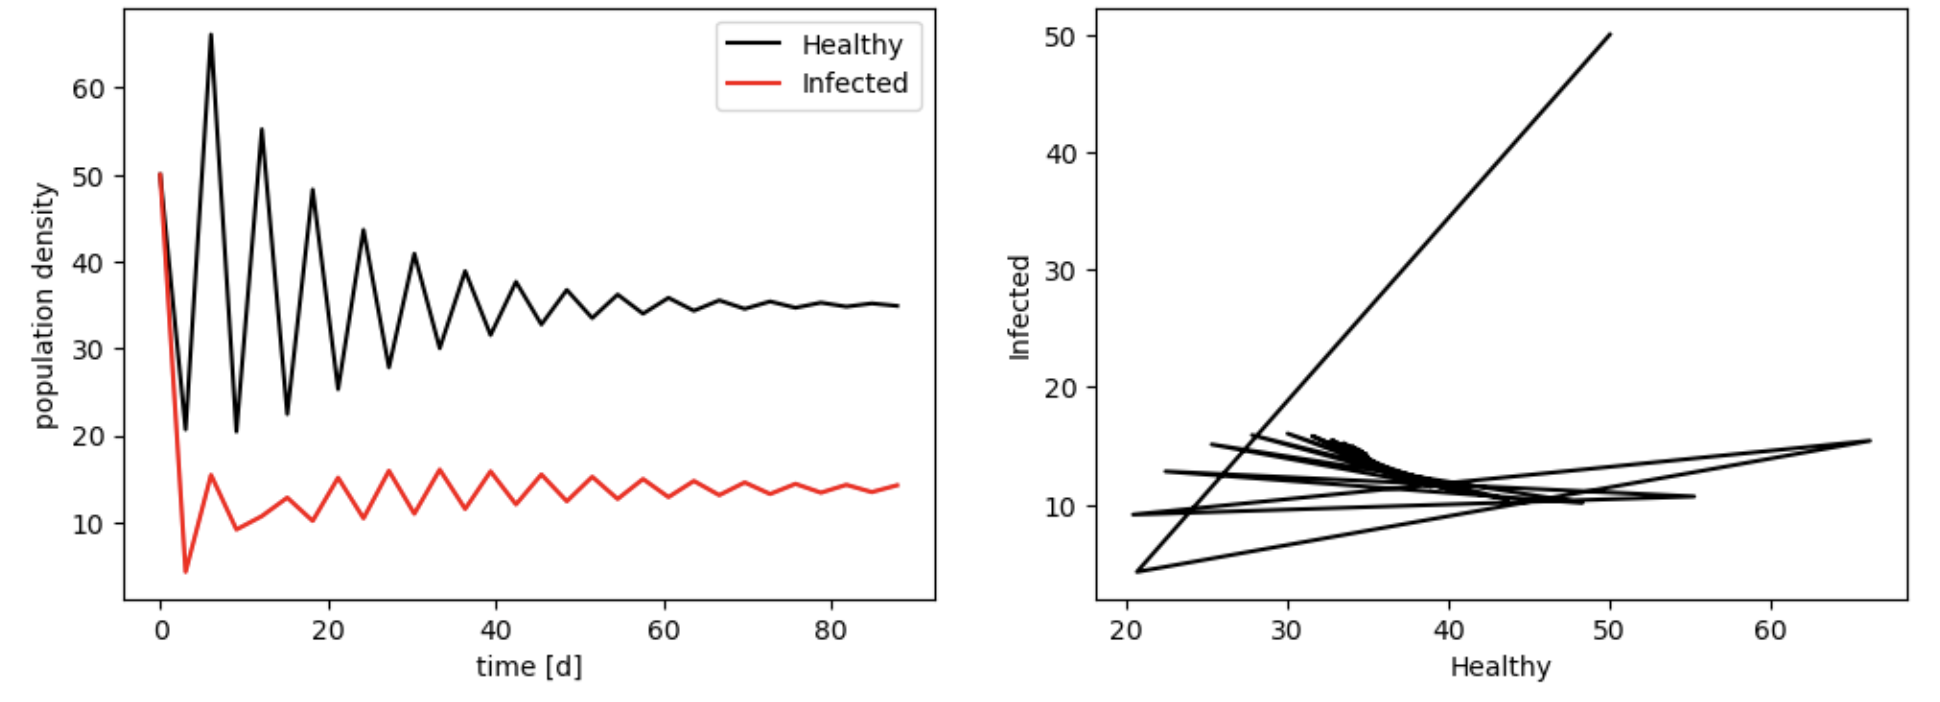
\includegraphics[width=16cm, height=5.2cm]{img/with_control.png}

\vspace{3mm}
\hspace{30mm} Figure 6. Vaccine, Treatments, and Five Controls

\vspace{3mm}

According to the CDC, 2 doses of monovalent mRNA COVID-19 vaccine were 36\% effective against COVID-19–associated hospitalization. Also, Sotrovimab, one of the COVID-19 treatments available, showed 79\% reduced chances of hospitalization. In this analysis, $\epsilon_H = 0.36, \epsilon_I = 0.79$ was used. for $u = [0.53, 0.11, 0.35, 0.41, 0.25]$, it represents border restriction, actively communicate with healthcare professionals, increase governmental support to vulnerable populations (41\%) and national lockdown (25\%) (Haug et.al., 2020).


Figure 6 demonstrates the interactions between healthy and infected populations in the presence of vaccines, treatments, and controls. The zig-zag shaped graph illustrates the behavior of the population with the implementation of controls. For instance, when the number of healthy individuals peaks, it decreases due to the infection, but it quickly recovers within a short time due to the implemented controls. Although the infection may continue to affect society over time, it stabilizes. Therefore, this analysis suggests that COVID-19 may not be eradicated, but the impacts on population numbers would be minimal. In other words, we will learn to coexist with COVID-19.
\pagebreak

\section{Discussions} \label{subm}
\hspace{5mm} The gLV model developed by Younes and Hasan (2020) provides a valuable framework for understanding how healthy and infected populations interact in an ecological perspective. While the lack of data on COVID-19 vaccines and treatments prevented the implementation of controls, setting $\epsilon$ to 0 still provided useful insights into how COVID-19 can affect human populations.

For example, the study concluded that the infection rate is a crucial factor for the interaction between healthy and infected populations. Figure 04 and Figure 05, which depict the impact of varying infection rates ($\beta$), further support this finding, as the higher infection rate in Figure 05 (0.05) led to a larger number of infected individuals compared to Figure 04 (0.005). Moreover, Figure 01 implies that if we had regulated travel or attempted to control the spread more strictly earlier, the pandemic might have ended earlier. With controls in Figure 06, it implies that COVID-19 might not disappear in the populations but live with us. As many experts argue from the early stage, the model also expected that infected populations will not diminish.

Compared to the statistical power series model described in section 2.2, the gLV model implemented controlling factors such as immigration and infection rate. However, the model's accuracy in predicting or simulating COVID-19 would have been enhanced if it could have incorporated the infection rates of various COVID-19 variants. To date, over 10 variants of COVID-19 have been identified, each with distinct death and infection rates. Incorporating this data could have further refined the model's predictions and given a more accurate representation of the spread and impact of the virus.

Another limitation of the gLV model is its computational constraints. The model can only simulate an arbitrary country with 100 people due to computational limitations. However, if computation is not an issue, utilizing real numbers from a specific country (such as the U.S.) could enable us to validate the model's accuracy.

One argument I will bring in is that the subject of the research did not necessarily need to be COVID-19. This model can be applied in any contagious disease. Of course, COVID-19 was the biggest pandemic happened in many years, and it is an ideal research topic to make the audience aware of what strategy we need to adopt. However, choosing COVID-19 was purposeful, and I have a feeling that the researchers want to get more attention by mentioning COVID-19. 

The paper by Younes and Hasan (2020) implemented the Extended Kalman Filter (EKF) to study the dynamics of infectious disease transmission. Unfortunately, due to time limitations, the present study was not able to explore this aspect in depth. However, it is worth noting that if EKF had been implemented in Section 2.4, the results might have been different. This is because EKF adds uncertainty to the dynamics of the system, which can have a significant impact on the outcomes. Therefore, future studies that implement EKF could provide a more accurate representation of the spread and impact of infectious diseases such as COVID-19.

Despite these limitations, the gLV model remains a valuable tool for understanding the dynamics of infectious disease transmission and the interactions between healthy and infected populations. With further refinement and incorporation of additional data, the gLV model may provide an even more accurate representation of the spread and impact of infectious diseases like COVID-19. This, in turn, could help inform public health policies and interventions aimed at mitigating the spread of infectious diseases and reducing their impact on human populations.
\pagebreak

\bibliographystyle{apacite}
\bibliography{contents/reference}

\end{document}

